% !TeX program = xelatex
\documentclass[UTF8,fontset=fandol,10pt,a4paper]{ctexart}
\usepackage[left=22mm,right=22mm,top=23mm,bottom=22mm,headheight=14pt]{geometry}
\usepackage{fontspec}
\setmainfont{TeX Gyre Heros}
\setsansfont{TeX Gyre Heros}
\setmonofont{Latin Modern Mono}
\renewcommand{\familydefault}{\sfdefault}
\usepackage[table]{xcolor}
\usepackage{graphicx,tikz}
\usetikzlibrary{arrows.meta,positioning,fit,backgrounds,calc}
\usepackage{booktabs,tabularx,array,enumitem,float,caption,fancyhdr,hyperref}
\definecolor{blue}{HTML}{2869A9}
\definecolor{ink}{HTML}{293340}
\definecolor{muted}{HTML}{647181}
\definecolor{line}{HTML}{C5D4E2}
\definecolor{pale}{HTML}{F0F5FA}
\definecolor{warm}{HTML}{FFF7E9}
\hypersetup{colorlinks=true,urlcolor=blue,linkcolor=blue,pdftitle={Redflag RHI 与 Vulkan 接入设计},pdfauthor={Redflag}}
\color{ink}
\setlength{\parindent}{0pt}
\setlength{\parskip}{6pt}
\linespread{1.16}
\setlist[itemize]{leftmargin=1.5em,itemsep=2pt,topsep=3pt}
\setlist[enumerate]{leftmargin=1.8em,itemsep=3pt,topsep=3pt}
\renewcommand{\arraystretch}{1.38}
\newcolumntype{Y}{>{\raggedright\arraybackslash}X}
\newcolumntype{L}[1]{>{\raggedright\arraybackslash}p{#1}}
\ctexset{section={format=\Large\bfseries\color{blue},beforeskip=16pt,afterskip=8pt},subsection={format=\large\bfseries\color{blue},beforeskip=11pt,afterskip=5pt}}
\captionsetup{font=small,labelfont=bf,textfont={color=muted},skip=7pt}
\pagestyle{fancy}\fancyhf{}
\fancyhead[L]{\small\color{muted}Redflag · RHI / Vulkan · 设计方案}
\fancyhead[R]{\small\color{muted}2026-11-21}
\fancyfoot[C]{\small\color{muted}\thepage}
\renewcommand{\headrulewidth}{0pt}
\newcommand{\note}[1]{{\small\color{muted}#1\par}}
\newcommand{\code}[1]{{\small\texttt{#1}}}
\newcommand{\ruleline}{\par\vspace{4pt}{\color{line}\hrule}\vspace{8pt}}
\newcommand{\source}[2]{{\small\href{#1}{[#2]}}}
\tikzset{
 module/.style={draw=line,fill=pale,rounded corners=2pt,align=center,inner sep=7pt,text width=3.8cm,minimum height=1.15cm,font=\small},
 smallbox/.style={module,text width=2.55cm,minimum height=.95cm,font=\footnotesize},
 wide/.style={module,text width=9.5cm},
 planned/.style={module,fill=warm,dashed},
 flow/.style={-{Stealth[length=2mm]},draw=muted,line width=.65pt},
 own/.style={flow,dashed},
 label/.style={font=\scriptsize,fill=white,inner sep=2pt,text=muted}}

\usepackage{amsmath}
\usepackage{fvextra}
\DefineVerbatimEnvironment{Code}{Verbatim}{fontsize=\small,breaklines=true,breakanywhere=true,frame=single,rulecolor=\color{line},framesep=6pt}
\hypersetup{pdftitle={Redflag 排错与 RenderDoc 截帧记录}}
\fancyhead[L]{\small\color{muted}Redflag · 排错与截帧}
\newcommand{\loc}[1]{\par{\footnotesize\color{muted}源码：\path{#1}}\par}
\renewcommand{\note}[1]{\par{\small\color{muted}#1\par}}
\setlength{\emergencystretch}{1em}
\begin{document}
\zihao{5}
\raggedright
{\Huge\bfseries Redflag 排错记录}\par\vspace{5pt}
{\Large\color{muted}问题、修改过程与 RenderDoc 截帧}\par
\ruleline

记录日期：2026-11-21。本文保存资源和渲染清理中确认的问题，也整理旧开发日志中的故障。每项都说明证据来自源码、自动测试还是历史记录。没有原资产和原现场的历史问题，不列为本轮复现成功。

本轮完成 Debug/x64 构建与下列基础回归，后续 3D 与 IBL 复查见第 \ref{sec:3d-review} 节。它们覆盖指定输入，还没有完成全部资产、整编辑器交互、长时间内存及 Release/Dist 回归。技术方案为什么这样选择、付出什么代价，另见《技术选型与工程取舍》。

另有一个 CPU 时间线采样用例，实际 Chrome 截图与采集条件放在选型文档。它不替代功能回归，也不是优化前后的性能对比。

\section{本轮验证范围}
\begin{tabularx}{\textwidth}{L{3.2cm}YL{2cm}}
\toprule
测试 & 检查的行为 & 结果 \\
\midrule
资产身份与缓存 & ID 持久化、移动、元数据错误、类型与外部引用。 & 通过 \\
Shader 与 GPU 对象 & 内容缓存、资源库查询，以及 VAO 的最后引用释放。 & 通过 \\
深度与主绘制 & 透明裁剪轮廓、实体 ID、关闭贴图后的状态更新。 & 六组通过 \\
模型导入 & 合并贴图尺寸、通道默认值，以及几何与法线保留。 & 十例通过 \\
后处理隔离 & 两实例曝光、交替绘制、尺寸变化、Bloom 与销毁。 & 通过 \\
\bottomrule
\end{tabularx}

GPU 测试通过 GLFW 创建隐藏的 OpenGL 4.6 上下文，在真实驱动上绘制并读回结果。修改生产代码后要先构建 Debug/x64，再从仓库根目录顺序运行测试，避免同时写入同一 Shader 缓存目录。

\begin{verbatim}
tests\run_asset_tests.cmd
tests\run_shader_tests.cmd
tests\run_depth_tests.cmd
tests\run_model_tests.cmd
tests\run_render_tests.cmd
\end{verbatim}

测试源码都在 \path{tests/}，对应文件为 AssetManagerTests、ShaderCacheTests、DepthPrepassTests、ModelImportTests 和 PostProcessTests。本机日志在 \path{tmp/comment-clarity/}，该目录不保证随仓库分发，复现应以测试源码与脚本为准。

构建日志 \path{build-final.log} 记录 Redflag 与 RedflagForge 编译链接成功。第三方 PDB 缺失、重复导入描述符和测试链接的增量调试选项警告仍在，构建成功不表示零警告。

\subsection{阅读与复查}
先看故障在什么输入下出现，再核对相关代码和测试。RenderDoc 截帧用于观察某次绘制真正拿到的数据与输出。自动测试负责把预期结果变成可重复的断言。旧日志只能提供排查线索，不能替代同一资产、同一设置下的复现。

\newpage
\section{Shader 编译与缓存}
\subsection{源码修改未使缓存失效}
\textbf{现象与定位。}原缓存按文件名区分 Shader，再用修改时间判断是否过期。不同目录的 \code{shared.glsl} 会指向同一份缓存。源码变了但时间戳不变，也可能继续执行旧代码。排错时即使改对了公式，画面仍可能不变。

\textbf{修改。}缓存改用阶段源码和编译配置的内容哈希，顶点与片元阶段分别保存。文件和字符串创建共用这条路径。读取时检查长度、完整读取结果及 SPIR-V 标记，截断文件会重新编译。同时删除没有读取方的第二阶段缓存写入，以及一处创建后未使用、未释放的 Program。

\textbf{验证。}测试实际绘制三角形。两个同名、同时间戳文件分别输出红色和绿色。修改源码但保持时间戳后输出蓝色。还检查字符串 Shader、三字节坏缓存，以及重复加载和只改时间戳时的缓存复用。所有断言通过。

\textbf{保留限制。}GLSL 450 路径只缓存第一阶段结果，后续反编译、再次编译和链接仍执行。配置键中的 \code{v1} 要随编译器或选项变化更新，尚未自动纳入版本与外部 include 依赖，也没有旧缓存清理。长度与标记检查不等于完整 SPIR-V 校验。这条中间代码路径服务于 OpenGL，Vulkan 后端尚未实现。
\loc{Redflag/src/Platform/OpenGL/OpenGLShader.cpp}

\subsection{GLSL 330 示例的普通 uniform 编译失败}
额外冷编译扫描最初有 15 个着色器成功，旧 FlatColor 示例失败。它用普通 uniform 传入矩阵和颜色，第二次中间代码编译却按 Vulkan 规则检查，拒绝了这些声明。修改编译目标还不足以证明按名称设置参数的旧接口仍正确。

GLSL 330 示例现交给 OpenGL 直接编译源码，保留 uniform 名称。GLSL 450 继续使用 SPIR-V，两条路径共用程序链接。合并主 Shader 之前，全部 16 个 .glsl 文件链接成功。FlatColor 按名称上传两个单位矩阵与颜色后，实际像素为 $(255,0,255,255)$。这检查了旧接口的使用结果，范围仍限于工程现有着色器与该绘制用例。

\newpage
\section{资源库查询与 GPU 对象释放}
\subsection{查找 Shader 意外插入空条目}
\textbf{现象与原因。}原 Get 对 Exists 的断言方向写反，会拒绝已经存在的名称。随后又通过下标查询，不存在的名称会被插入库中，留下一个空对象。

\textbf{修改与验证。}Get 改为 \code{m\_Shaders.at(name)}。测试确认 Add 后取得同一个对象。缺失名称抛出\allowbreak\ \code{std::out\_of\_range}，随后 Exists 仍为 false。调用方必须遵守先登记再查询的约定，查询本身不创建资源。
\loc{Redflag/src/Redflag/Renderer/Shader.cpp}

\subsection{VAO 对象泄漏}
\textbf{现象与原因。}OpenGLVertexArray 构造时创建了顶点数组对象（VAO），析构函数却为空。缓冲引用虽然释放，VAO 没有对应删除调用，这是源码可以确认的 GPU 对象泄漏。

\textbf{修改与验证。}析构调用 \code{glDeleteVertexArrays}。测试取得真实对象 ID，释放一个共享引用时对象仍存在，最后一个引用释放后 \code{glIsVertexArray} 返回 false，且没有 GL 错误。释放仍必须发生在有效上下文内。本轮验证了删除行为，没有测量长期显存变化。
\loc{Redflag/src/Platform/OpenGL/OpenGLVertexArray.cpp}
\note{API 依据：\source{https://registry.khronos.org/OpenGL-Refpages/gl4/html/glDeleteVertexArrays.xhtml}{Khronos：glDeleteVertexArrays}。}

\newpage
\section{材质透明裁剪不一致}
树叶、围栏这类裁剪材质，会用贴图透明度丢弃部分像素。原深度预传递只读取独立透明度图或底色因子，主绘制还会读取底色贴图的透明通道。主绘制丢弃的像素可能已经写入深度和法线，继续影响后续遮挡计算。

\subsection{统一材质输入与裁剪规则}
Mask 表示按阈值保留或丢弃像素。深度预传递现在复用主绘制的材质上传，取得相同的底色与独立透明度贴图，按下式计算透明度：
\[
\alpha=\alpha_{\text{底色因子}}
       \times\alpha_{\text{底色贴图}}
       \times r_{\text{透明度贴图}}.
\]
没有对应贴图时，该项按 1 处理。低于材质阈值的像素丢弃，Opaque 材质不做这项裁剪。两次绘制必须读取相同的材质透明度，仅检查纹理已经传入还不够。

\subsection{独立绘制与覆盖率验证}
测试把 32×32 目标分成四条纹，逐项启用底色 alpha、独立 AlphaMap 和二者相乘。其他输入检查仅底色因子、Opaque 不裁剪，以及复用队列后关闭贴图。

深度预传递和主绘制各自清屏、独立绘制，再逐像素比较深度覆盖与实体 ID。这样预传递留下的深度不会遮住主绘制本身的错误。六组输入全部通过。

\textbf{验证边界。}这组测试覆盖深度预传递和普通主绘制。阴影与 RSM 的新增测试见第 \ref{sec:3d-review} 节，仍未覆盖完整场景中的全部透明路径。RenderDoc 的实际截帧见后文，不能把这一个最小场景扩大为所有效果都已回归。

\loc{RedflagForge/assets/shaders/Depth_Prepass.glsl}
\loc{Redflag/src/Redflag/Renderer/Renderer3D.cpp}
\loc{tests/DepthPrepassTests.cpp}

\subsection{排查顺序}
画面出现多余遮挡时，先比较颜色输出与深度覆盖。轮廓不同，再检查这两次绘制使用的裁剪公式、贴图内容和材质开关。将错误缩小到四条纹输入后，就能区分是贴图未传入、状态没有刷新，还是透明度计算不同。修复后的断言保留每种输入，避免只凭最终画面判断。
\note{参考：\source{https://learnopengl.com/Advanced-OpenGL/Blending}{LearnOpenGL：丢弃透明像素与混合}。该教程解释 Mask 与半透明混合的区别，本项目的三项乘积由实际材质约定决定。}

\newpage
\section{模型导入与材质误判}
\subsection{金属度和粗糙度贴图尺寸不同}
\textbf{现象与原因。}原合并函数发现尺寸不一致后只打印警告，随后仍按金属度图的尺寸遍历两张图。粗糙度图更小时可能越界。即使像素总数一样，长宽不同也不能认为同一数组下标代表相同纹理位置。

\textbf{修改。}尺寸不一致就拒绝合并，释放临时像素并返回空纹理，材质继续使用标量参数。本次没有加入重采样，也不猜测两张贴图该怎样对齐。

\textbf{验证。}测试生成 OBJ、MTL 和 TGA 后真实导入，覆盖尺寸一致、任一图更小、总像素相同但形状不同，以及缺一张或两张图的输入。合并成功时读回 GPU 纹理，检查通道为 R=0、G=粗糙度、B=金属度、A=255。缺粗糙度时为 128/255，缺金属度时为 0。三种尺寸错误均不生成合并纹理。

这些断言证明测试输入在合并前被拒绝，没有进行地址消毒器或随机损坏文件测试。

\subsection{默认透射色被当成玻璃证据}
\textbf{实际发现过程。}最初七例只检查贴图合并，全部通过，日志里却出现了不该有的玻璃判断。继续检查发现，未声明透明的最小 OBJ 已被清空 MeshData。贴图生成正确，掩盖了模型几何被删除的问题。

\textbf{原因。}项目携带的 Assimp 把 OBJ 透射颜色默认设为 $(1,1,1)$，并写入透明色属性。原 Model 将非零透射色视为透明度证据，直接清空子网格。同一段代码还根据材质名、网格名或路径里的 glass、window、mirror 猜测材质，附带修改金属度/粗糙度或移除法线图。这些字符串不能代替材质声明。

\textbf{修改。}删除整段名字、路径和透射色猜测，以及删除几何、改参数、清法线的副作用。普通材质保持 Opaque，显式加载独立 AlphaMap 时进入 Mask。没有补做 Blend 导入或半透明排序。

\textbf{验证。}测试当时扩为九例，每例都检查 MeshData 非空。新增 glass 材质名与 mirror 路径，确认法线仍在，底色为白色，金属度为 0，粗糙度为 0.5。九例通过，后续显式材质因子用例再扩为十例。导入测试应同时核对几何与材质，避免单项结果掩盖其他损坏。
\loc{Redflag/src/Redflag/Renderer/Model.cpp}
\loc{tests/ModelImportTests.cpp}
\note{依赖依据：当前 Assimp 副本 \path{code/ObjFileData.h:193} 与 \path{code/ObjFileImporter.cpp:601}。这说明当前依赖的行为，不推广到所有版本和格式。}

\newpage
\section{资源重构中已经修正的问题}
以下变化可在提交 \source{https://github.com/caihongqiu417/RedflagEngine/commit/1a168c380fbf3942cb7028000d0fef92c3848a1b}{1a168c3} 中追踪。本轮再次运行资产和后处理测试，其他生命周期修改仍以源码核对为主。

\subsection{移动文件后丢引用，卸载后又自动加载}
模型曾只按路径保存身份，移动后旧路径无法表达它仍是同一份资产。现在模型旁的 .rfmeta 保存稳定 ID，AssetLibrary 记录 ID 到路径的对应，AssetManager 按 ID 缓存。源文件和元数据一起移动，重新扫描后仍可按原 ID 找到。旧场景的 FilePath 在读取时转换为 ID。

卸载模型除了移除缓存，还清空组件的 ID、路径和覆盖材质。只删缓存、留下加载来源，会使后续渲染再次加载。外部仍持有 Ref 时资源继续有效，Unload 或 ClearAll 只释放缓存自己的引用。

资产测试覆盖持久化、移动与路径别名，也包含 Windows 大小写路径、坏元数据、重复 ID、类型错误和加载失败重试。失败扫描不会替换有效库。本轮通过的是测试资产，尚未替代完整场景交互。任意移动 assets 外文件也不能保证自动找回。
\loc{Redflag/src/Redflag/Assets/AssetLibrary.cpp}
\loc{Redflag/src/Redflag/Assets/AssetManager.h}

\subsection{GPU 资源释放与退出顺序}
退出顺序现在明确为停止并销毁 Layer、关闭脚本、清空资产缓存和资源库、关闭 Renderer，最后销毁窗口。LayerStack::Clear 执行 OnDetach。移除 Overlay 不再错误减少普通 Layer 插入索引。

GPU 删除依赖有效上下文，仅让对象最终析构还不够，必须控制最终引用释放的时机。本轮核对了源码和构建，还没有对所有 Play/Simulate 退出路径做交互压力测试。
\loc{Redflag/src/Redflag/Core/Application.cpp}
\loc{Redflag/src/Redflag/Core/LayerStack.cpp}

\subsection{后处理实例状态隔离}
原先，场景绘制代码统一处理 Bloom 和最终颜色。现在每个 PostProcess 实例都管理自己的着色器、渲染目标、全屏绘制资源，以及存放曝光值等设置的缓冲区。这些资源随实例创建和释放。用两个实例交替绘制时，即使新的曝光值已经写好，着色器也可能还在读前一个实例的设置。绘制前需要把着色器切换到当前实例的缓冲区。

测试给两个实例不同曝光，交替绘制后第一个结果保持不变。调整其中一个的尺寸不影响另一个，Bloom 开关、输出和销毁检查也通过。这只证明后处理实例隔离，整个 SceneRenderer 的阴影、SSAO 与 RSM 仍有静态状态。
\loc{Redflag/src/Redflag/Renderer/PostProcess.cpp}
\loc{tests/PostProcessTests.cpp}

\newpage
\section{3D 绘制路径复查}\label{sec:3d-review}
这次复查从同一个物体在不同绘制阶段的行为入手。以下数值来自独立 GPU 测试，原有 RenderDoc 捕获仍只对应深度预传递与普通主绘制，不能代替本节新增证据。

\subsection{屏幕外物体被一并移出阴影}
原先在主相机视锥外就丢弃绘制命令。相机看不到的物体仍可能处在光源范围内，给可见表面投下阴影或贡献 RSM 数据。过早删除命令，会让这些影响一起消失。

现在保留提交内容，主相机的深度预传递与主绘制按相机可见性筛选，Shadow 与 RSM 仍处理该物体。测试把四边形移到相机外，再调整光源矩阵使其落在光源范围内。主画面不写深度，阴影深度和 RSM 表面数据仍出现，绘制次数也与预期一致。另检查相交边界和负缩放包围盒。
\loc{Redflag/src/Redflag/Renderer/Renderer3D.cpp}
\loc{tests/Renderer3DTests.cpp}

\subsection{阴影与 RSM 的透明裁剪缺项}
修复普通主绘制和深度预传递后，阴影与 RSM 仍需逐条核对。它们此前没有使用完整的底色因子、底色贴图 alpha 与透明度图红通道乘积，会留下本该裁掉的遮挡面。

现在三项输入共用同一材质上传规则。Renderer3DTests 对 $32\times32$ 的四条纹逐像素检查 Shadow 深度和 RSM 深度、表面有效标记。Mask 只保留两侧，Opaque 保留全部，Blend 仍跳过这两个光源绘制阶段。测试通过不表示半透明投影已经实现。
\loc{RedflagForge/assets/shaders/ShadowDepth.glsl}
\loc{RedflagForge/assets/shaders/RSMDepth.glsl}

\subsection{普通与实例化主绘制的光照不一致}
两份主 Shader 曾分别维护光照，实例化分支可能遗漏普通路径已经加入的 RSM 输入。现在用同一个源码和实例化编译选项组织两种顶点输入，片元光照共用实现。

测试输入固定红色间接光，普通与实例化输出的红通道都增加 0.5，绿蓝不变。实例化用一次绘制写出左右实体 ID 71、72。这证明指定输入下两条路径读取了相同的间接光规则，没有测量性能提升。当前是 15 个 .glsl 文件，另编译一个实例化版本。
\loc{tests/DepthPrepassTests.cpp}

\subsection{RSMDepth 的跨阶段参数块重名}
新测试第一次链接失败时，顶点和片元阶段各自生成了临时名 \code{\_11\_13}，实际内容却分别是模型矩阵与材质参数。链接器将同名块视为同一声明，产生冲突。这次问题有实际链接失败记录，与旧 varying 名称问题不同。

反编译阶段现在按资源绑定位置统一命名块类型与实例，使同一份数据名称一致、不同数据名称不同。修复后 Shader 链接与 Renderer3D 逐像素测试通过。这个规则服务当前 OpenGL 布局，不是 Vulkan 后端已完成的证明。
\loc{Redflag/src/Platform/OpenGL/OpenGLShader.cpp}

\newpage
\section{导入数据与 IBL 资源复查}
\subsection{显式零值被当成缺失参数}
旧导入逻辑会在有贴图时将接近黑色的底色改白，并把零金属度、零粗糙度视为没有提供参数。零是合法材质值，不能用数值本身判断属性是否存在。

现在根据 Assimp 查询是否成功区分缺失与显式值，保留黑色、底色 alpha 和两个零因子。新增 glTF 用例同时给出白色贴图与 $(0,0,0,0.25)$ 底色，以及金属度、粗糙度零值，导入后逐项断言保留。模型测试因此从九例扩为十例。无对应贴图且属性缺失时仍使用金属度 0、粗糙度 0.5，有贴图而缺少乘数时使用 1。

这验证的是导入数据不被猜测覆盖。材质仍没有完整 Blend 导入与排序，保存 alpha 不能被描述为玻璃已经正确显示。
\loc{tests/ModelImportTests.cpp}

\subsection{IBL 预计算与绘制状态}
预计算和全屏后处理会在场景绘制之间运行。继承剔除、裁剪或拒绝所有片元的深度状态，会使预计算输出为空。现在显式设置必要状态，结束后恢复。IBLTests 故意设置这些状态，再执行真实 HDR 预计算，检查产物和调用后状态。

另一条失败路径在 HDR 读取前就创建辅助四边形，Shutdown 却没有删除它。现在成功解码后才分配，删除无调用方的空环境准备接口，Shutdown 同时释放四边形与立方体资源。

测试使用常量 HDR $(2,1,0.5)$，读取环境图与辐照度图的六面，以及预过滤图五个 mip 层。颜色在容差内保持一致，BRDF 查找表为有限值且有有效输出。预计算后 viewport 与相关绘制状态恢复，Shutdown 后产物纹理和辅助 VAO/VBO 不再有效。缺失文件也保持未就绪并释放资源。

后处理测试另在剔除全部面、只允许 $1\times1$ 裁剪区域的条件下绘制，确认完整目标仍有均匀输出，调用后保留外部开关。原有双实例曝光和尺寸检查继续通过。测试只覆盖所列状态与输入，没有做全部 GL 状态组合或长时间压力测试。
\loc{tests/IBLTests.cpp}
\loc{tests/PostProcessTests.cpp}

\subsection{纹理上传的行对齐}
宽度为 3 的 RGB 图每行有 9 字节，文件解码数据紧密排列，默认四字节对齐却会让下一行从错误位置开始。上传现在临时使用一字节对齐，完成后恢复调用者原值。文件加载和 SetData 使用相同约定，并补齐灰度、灰度加 alpha 的格式与采样分量。

测试对 $3\times2$ 的 1、2、3、4 通道图分别上传、修改并逐像素读回，进入时刻意把对齐设为 8，结束后仍为 8。全部通过。这是新生成素材的结果，不据此给早年棋盘倾斜补写根因。
\loc{Redflag/src/Platform/OpenGL/OpenGLTexture.cpp}

\newpage
\section{场景帧与附件状态复查}
\subsection{深度附件查询与预览}
主目标使用纯深度 DEPTH32F，SSAO 和 RSM 却查询深度模板组合附件。现在统一查询深度附件。深度预览同时修复上传行对齐的恢复，以及整张图只有一种几何深度时显示为空的处理。Shutdown 清掉借用的纹理 ID，避免面板继续使用失效名字。

SceneRenderTests 在编辑和运行路径连续绘制，确认 SSAO/RSM 不产生 GL 错误，历史输出存在，预览中单深度平面可见，销毁后查询返回零。这里验证附件接通和状态，不评价复杂场景的遮蔽效果或历史拖影。

\subsection{跨帧 2D 混合与方向光选择}
后处理关闭混合后，下一帧 2D 没有重新启用，半透明精灵会失去预期混合。场景现在在 2D 阶段设置标准 alpha 混合，在 3D 数据阶段关闭混合，并避免 2D 向法线附件写入未定义值。连续帧测试读到预期的 0.5 颜色和零法线。

方向为零的灯光也曾先归一化再判断，可能产生 NaN。现在先检查向量，再上传有效灯光。主绘制只支持一盏方向光时，阴影必须跟随实际上传的同一盏，不能另找后面的可投影灯。测试分别检查零方向不上传，以及当前灯不投影时阴影关闭。
\loc{tests/SceneRenderTests.cpp}

\subsection{天空盒串写实体号和法线}
这次实测先把实体附件清为 -1、法线首分量清为 0.25，画天空盒后分别变成 1073741824 和 2。天空盒 Shader 只声明颜色输出，但其余附件仍允许写入，不能依赖未声明输出替自己保留旧数据。

修复在天空盒绘制期间关闭实体号和法线附件的写入，再恢复原掩码。最终测试保留 -1 与 0.25，也检查此前颜色写掩码没有改变。它避免天空背景污染拾取与 SSAO 输入，没有增加天空盒参与这些附件的含义。
\loc{Redflag/src/Redflag/Renderer/IBLPrecompute.cpp}
\loc{tests/IBLTests.cpp}

\subsection{复现入口与最终记录}
最终 Debug/x64 构建及八组回归全部通过。新增三组从仓库根目录运行，基础五组仍使用前文脚本。
\begin{verbatim}
tests\run_renderer3d_tests.cmd
tests\run_ibl_tests.cmd
tests\run_scene_tests.cmd
\end{verbatim}
失败与八组通过记录已节选到 \path{output/validation/opengl-regression.txt}，可随仓库复查。本机完整日志为 \path{tmp/comment-clarity/verified-*.log}。15 个 .glsl 独立链接通过，实例化版本另有实际绘制断言。这些专项结果仍不能替代完整编辑器交互、所有资产和长期压力测试。


\newpage
\section{RSM 通量与采样范围修正}\label{sec:rsm-energy}
经典场景仍出现不合理的间接光后，继续调强度难以判断问题来自哪里。前轮测试已经证明 RSM 附件接通、普通与实例化都读取它，但这些检查没有证明反射光的数值正确。本次先拆开通量写入、间接光收集和接收材质，分别与解析结果比较。

\subsection{从距离衰减排查到面积缺失}
原论文的几何因子分母是距离四次方，项目则是距离平方。逐项展开后发现，论文的两个点积使用未单位化的位移，各带一次距离。项目先单位化，因此这两种写法等价。距离平方本身不是错误。

真正不一致的是 RSMDepth 把底色、光强与入射余弦相乘，称为通量，收集阶段又只对样本求平均。方向光的一个纹素代表固定投影面积，倾斜表面的实际面积增长恰好抵消入射余弦。旧实现既多乘了该余弦，也没有把采样圆盘面积计入结果。强度倍率会掩盖其中一部分亮度差，无法恢复正确的尺度关系。

现在附件保存按光源投影面积计的反射通量密度，收集时统一乘圆盘投影面积，并计入发送、接收两端的 Lambert 系数。收发材质都使用 $(1-\text{metallic})\,\text{albedo}$，使纯金属不再参与这项漫反射。完整推导与旧提交 \code{1a168c3} 的最短代码对照放在《渲染公式与实现》的 RSM 节。

\subsection{采样数量不再缩小覆盖范围}
原始圆盘按 128 个点生成，却只取用户请求的前 N 个。前面的点更靠中心，减少到 16 个时覆盖半径只剩约 35\%。现在按实际 N 生成等面积圆盘，参数变化时清除旧历史，避免继续混入旧设置的结果。

固定的距离偏移和贡献上限改为一个光源纹素宽度的最小距离。它随场景覆盖尺度变化，但仍是近距离近似。圆盘外或没有表面的样本贡献为零，分母保留请求样本数，不按有效数量重新放大。

\subsection{实际验证与剩余限制}
Renderer3DTests 分别检查圆盘面积、距离翻倍的衰减、相同世界采样半径的结果、正照与斜照，以及背面和纯金属发送端。DepthPrepassTests 检查纯金属接收端。两组真实 GPU 数值测试通过，具体输入与误差列在公式文档。

两反射点之间仍没有可见性查询，挡板后的漏光属于尚未实现的遮挡处理。当前只有一次间接漫反射，历史也没有物体运动与前帧深度拒绝。新公式通过不能扩大成复杂场景全部正确，经典场景的图片与对照另见《经典场景实测》。

\loc{RedflagForge/assets/shaders/RSMDepth.glsl}
\loc{RedflagForge/assets/shaders/RSMIndirect.glsl}
\loc{Redflag/src/Redflag/Renderer/SceneRenderer.cpp}
\note{依据：\source{https://users.soe.ucsc.edu/~pang/160/s13/proposal/mijallen/proposal/media/p203-dachsbacher.pdf}{Dachsbacher、Stamminger：Reflective Shadow Maps，§3，印刷页 204--205}。验证记录见 \path{output/validation/rsm-regression.txt}，场景对照在 \path{output/scenes/rsm/}。旧 Mask 的 RenderDoc 捕获不用于证明此次 RSM 数值。}


\newpage
\newcommand{\rev}[1]{\source{https://github.com/caihongqiu417/RedflagEngine/commit/#1}{#1}}
\section{图集取错颜色、部件重叠与跨窗拖拽}
下面几页把旧场景的问题按当时的线索重走一遍。日志能告诉我们作者最初看到了什么，提交能告诉我们实际改了哪一行。这批旧问题都没有保留下当时的 RenderDoc 帧。

\subsection{Kenney 模型的一部分采到了黑色}
Kenney 模型用一张图集给不同部位上色，导入后却有一片变黑。旧日志沿图片和纹理坐标两头检查：图片加载时已经上下翻转，Assimp 又启用了 \code{aiProcess\_FlipUVs}。修复保留图片加载时的翻转，去掉导入模型时的第二次处理，让模型重新取到图集中对应的色块。

如今 Model 仍未启用这个 Assimp 标志。原 Kenney 资产本次没有重载，其他格式需要根据图片来源和 UV 约定分别验证。
\note{依据：\path{Task/ModelImport_DevLog.md} 第 2 节；导入提交 \rev{3bcd608}。}

\subsection{子网格叠在原点}
多部件模型加载后，明明有几个子网格，画出来却都叠在原点。ProcessNode 递归找到了孩子节点，却漏了从父节点走到当前节点时应乘的变换。修复把父节点与当前节点的矩阵累积到 SubMesh::LocalTransform，绘制时再乘整个实体在场景里的变换。

父子矩阵这条乘法链在提交和当前源码中都能找到。多层节点的专用资产回归仍然缺失；前文的材质用例检查几何有没有被删，未检查层级位置。
\note{依据：同一日志第 6.1 节；提交 \rev{f433b7e}；Model::ProcessNode、Renderer3D::DrawModel。}

\subsection{加入 3D 后，2D 场景全黑}
旧日志里，3D 加入后，原本能画出的 2D 场景变黑了。先查相机。3D 初始化选中了自己的相机数据，随后 2D 即使更新了自己的矩阵，着色器仍可能读 3D 的那份。再查真正绘制的地方，2D 的 Flush 也没有选回自己的着色器和顶点数组。

修复让更新相机时选回对应的数据，提交精灵时选回 2D 程序与顶点数组，并在初始化时恢复贴图数组。两套相机的内存各自存在，错的是绘制当刻所选的对象。后处理双实例测试复现过相似的状态切换，当年的完整 2D 场景没有在本轮重建。
\note{依据：同一日志第 6.2 节；提交 \rev{0e46596}。}

\subsection{跨窗口拖拽中断}
从资源浏览器把图标拖向另一个窗口，鼠标一离开图标，目标窗口就接不到路径。旧日志记下四次尝试：先依赖鼠标悬停，后来改看图标是否活动。拖拽系统接管之后，这两种状态都可能消失。直接调用 BeginDragDropSource 也仍会中断。

最终在鼠标按下时记住资源路径和类型，按住期间由窗口持续用 SourceExtern 发布数据，松开后再清空。ContentBrowserPanel 至今保留这几个成员。这里能对照当时的尝试和当前实现，尚未重测各种跨窗口布局。
\note{依据：同一日志第 3 节 ContentBrowserPanel 的迭代表；当前 ContentBrowserPanel.cpp。}

\newpage
\section{播放时消失的灯和环境图上的黑块}
\subsection{复制场景遗漏灯光和运行时网格}
编辑场景切到运行，方向光、点光源或程序生成的网格可能缺席。查看提交 \rev{3a5c63a}，Scene::Copy 与 DuplicateEntity 的复制清单原先漏了两类光，RenderRuntime 则漏了遍历程序网格。修复分别补齐复制和绘制。

当前源码仍含这两项处理。原提交没有失败画面和自动测试，无法确定当时先看见灯消失，还是先看见模型消失。

\subsection{停止播放后，变换手柄还拿着旧实体}
在播放中选中一个实体，然后点停止。编辑器在这一帧换回编辑场景，但稍后绘制的变换手柄（Gizmo）手里还拿着运行场景的实体。修复把播放时写入选择、操作手柄的入口限制住，防止运行时副本留在编辑状态里。这个过程来自提交说明和代码，全部 Play/Simulate 组合仍未做交互压力测试。
\note{依据：提交 \rev{4c3140b}；ForgeLayer 的鼠标选择与 Gizmo 分支。}

\subsection{环境光图上的黑块从哪里开始}
环境光照的结果是一片黑时，老指南先把漫反射环境图、不同粗糙度下的环境图和 BRDF 查找表分别显示。哪张先出黑块，就从哪张往回看；若读到 NaN，再用颜色标出来源，最后检查输入 HDR。提交 \rev{846e3de} 写的是 NaN 修复，原来那张 HDR 的出错像素和截帧都没留下。

当前代码把 NaN、无穷大等非有限输入改成零，有限亮度限制到 $[0,50]$。这会削弱特别亮的环境光源。旧文中“Inf 求平均必然变 NaN”的解释并不准确，结果还取决于随后做了哪些运算。
\note{依据：\path{Task/IBL_Implementation/IBL_Implementation_Guide.md} 第 10.3、20、21 节；IBLPrecompute.cpp。}

\subsection{粗糙反射的亮点与随相机移动的天空盒}
指南把这些现象分开检查，而不是统一归咎于光照公式。纹理还没有 mip 层就启用 mip 过滤，会使采样条件不完整。修复先使用普通线性过滤，生成层级后再切换。粗糙反射出现亮点，则检查采样与亮源分布，预过滤使用概率密度选择读取的 mip 层。

天空盒用到的立方体在预计算结束后还要继续绘制，因此它的顶点数组要留到 Shutdown。观察矩阵只取旋转，相机平移时天空仍在远处；使用正交投影则跳过天空盒。旧指南还列出六个面的朝向、环境光开关和 BRDF 的几何项。关于这几项，只留有检查建议。

旧照片没有逐项保留下来。前面提到的常量 HDR 测试是后来补做的，用来核对当前预计算。
\note{依据：同一指南第 11、14、18、20、21 节；提交 \rev{846e3de}、\rev{56cacd6}。}

\newpage
\section{灯光读错、泛光重复滤波与环境遮蔽条纹}
\subsection{同一盏灯的颜色和位置读偏了}
旧管线文档记录了一盏读错颜色与位置的灯。C++ 一连放三个 int，只占 12 字节，而着色器把同样的填充写成了 \code{int pad[3]}。按 std140 规则，这类数组的相邻元素间隔 16 字节。于是两端从不同位置开始读下一盏灯。

当时改用三个独立标量作填充，按灯光头 16 字节、每盏灯 64 字节核对。文档与提交保存了写法和改动。原始数据没有保留下来，现在的灯光参数检查只能独立验证当前布局。
\note{依据：\path{Task/RenderPipeline_Doc.md} 第 6 节及 std140 附录；提交 \rev{9e5f194} 的灯光声明。}

\subsection{顶点输出与片元输入在链接时对不上}
顶点着色器送出一个值，片元着色器接收它，两段程序在链接时需要对得上。老管线日志记录了一次中间代码转换后两侧名称不一致的问题。现在的反编译步骤根据相同的 location 生成相同的名字，再编译、链接。

仓库没有保留下来那次链接错误原文和最小失败 Shader，因此不能补写具体驱动报错。当前工程链接与像素测试另有结果，历史名称问题与本轮 GLSL 330 的 uniform 问题也不是同一错误。
\note{依据：同一文档第 11.2 节；OpenGLShader.cpp 中的 renameByLocation。}

\subsection{泛光已经合好，最终画面又滤了一遍}
泛光是先缩小图像提取亮部，再逐级放大、把亮度合回去。查看提交 \rev{dc1457c}，上采样已经把各层合到第一层，最后画到屏幕时又做了一次九点滤波。修复删掉这个额外步骤，直接采样合好的泛光图。当时没有记录误差数值，单凭这段代码也推不出每处边缘都会变硬。

同一提交为 2D Quad 和 Circle 增加颜色到线性空间的近似转换，使写入 HDR 与最终显示转换遵守同一流程。它还把清屏色改成黑色，但没有独立实验说明这项对故障的贡献。本轮后处理测试验证开关、隔离和输出，不是原图的前后视觉对比。
\note{依据：同一提交的 Composite、2D Shader 与 ForgeLayer 差异。}

\subsection{SSAO 重复条纹与采样方向}
屏幕空间环境遮蔽（SSAO）沿表面法线周围选方向取样。如果整面墙使用同一组方向，误差也会沿相同方向排成条纹；若用来生成方向的固定轴正好与法线平行，叉乘还可能变成零。旧实现改为从一张 $4\times4$ 噪声图取方向，去掉沿法线的分量，在每个像素建立自己的切线方向。

提交 \rev{82989dd} 保存了这次改动。当前仍用噪声旋转，没有额外加一遍模糊。增加采样和保留噪声之后的花费，旧记录里缺少同场景的时间或图像指标。随机选方向也仍可能偶遇与法线几乎平行的向量。
\note{依据：\path{Task/SSAO_Implementation_Doc.md} 第 3、6 节；\source{https://learnopengl.com/Advanced-Lighting/SSAO}{LearnOpenGL：SSAO}。}

\newpage
\section{阴影条纹、离地亮缝与间接光拖影}
\subsection{从条纹和亮缝判断该往哪里查}
旧阴影指南把几种看起来相似的瑕疵画在同一张速查表里。黑条纹和离地的亮缝都与深度比较有关，却不能照同一个方向调参数。原日志没有注明表中每一项是否都在 Redflag 复现过，下表据此保留检查步骤。

\noindent\begin{tabularx}{\textwidth}{L{3.3cm}Y}
\toprule
现象 & 日志建议的检查与取舍 \\
\midrule
受光面出现黑条纹 & 对照灯光深度与当前表面，检查深度精度和 bias；增加偏移也可能让阴影离开物体。 \\
阴影与物体间有亮缝 & 检查偏移是否过大，逐项调整，不能同时扩大多个参数后只看最终画面。 \\
场景边缘没有阴影 & 核对光源覆盖范围。扩大正交范围会降低同一张 ShadowMap 的空间精度。 \\
阴影锯齿或模糊 & 区分纹素分辨率与滤波半径。PCF 比较邻近深度后平均遮挡结果。 \\
PCSS 全部显得很软 & 检查光源尺寸与半影计算；原指南没有该参数的自动校准或前后测量。 \\
已有深度但主绘制无阴影 & 先确认主 Shader 读取的是这张图，再检查投影和范围，不先调亮度掩盖问题。 \\
\bottomrule
\end{tabularx}

指南还记载只使用一张方向光阴影图，以及当时跳过透明材质。前者不能由“增加级联”自动变成多灯光阴影。级联解决的是同一方向光在不同距离的覆盖和精度。透明裁剪是否正确则必须分别检查阴影、深度和主绘制，本轮新增验证另列。
\note{依据：\path{Task/Shadow_Implementation_Guide.md} 第 8、9、19、21 节；提交 \rev{56cacd6}；\source{https://learnopengl.com/Advanced-Lighting/Shadows/Shadow-Mapping}{LearnOpenGL：Shadow Mapping}。}

\subsection{用上一帧的光减轻间接光锯齿}

提交 \rev{70f2dd3} 想减轻间接光的锯齿，把本帧间接光与上一帧的颜色分开保存。现在先用当前深度还原表面的位置，再去上一帧对应的位置取颜色，并用周围像素限制旧颜色的范围。原提交没有保留对照截图或测量值，无法从记录中看出镜头停下后还有多少噪点，也看不出移动时物体边缘的拖影有多长。
这条修复开始用上一帧平滑间接光。原先标题里用过 TAA 一词，当前实现仍缺少物体运动信息和前一帧的表面深度对照。新露出的墙面可能把先前遮住它的物体颜色带进来。

\subsection{有白色贴图的黑材质曾被改白}
旧管线文档曾为一批 FBX 写下补丁：有底色图、底色又很暗，就把底色改成白色。作者明确把材质设为黑色时，这条规则同样会触发。早先根据 glass、mirror 等名字移除网格的处理也有类似问题。

现在改查文件是否真的提供了这些属性，保留取值为零的材质。前面用一张白图和一个黑色材质作对照的 glTF 用例，正是在复查这项旧补丁。
\note{依据：\path{Task/RenderPipeline_Doc.md} 第 10 节的 FBX 修复说明；Model.cpp 历史与本轮差异。}

\newpage
\section{精灵残留、视口拉伸与鼠标误操作}
这组提交早于 3D 管线。它们保留了问题和改动，缺少原始截帧及系统复测，因此不能替当前编辑器完整回归。

\subsection{空批次仍触发绘制}
提交 \rev{e80839c} 检查一帧结束时有没有精灵真的提交。原来空批次也上传顶点并 Flush，底层 DrawIndexed 恰好把零理解为使用整个索引缓冲，旧顶点于是有机会又画一次。现在本批索引数大于零才提交。文末保留了当时的代码。这项历史修复缺少原截图与空帧切换的专用回归。

\subsection{视口缩放使相机比例失调}
提交 \rev{783d448} 增加 SceneCamera::SetViewportSize，并在视口变化时通知不固定比例的相机，重新计算投影。差异确认处理的是投影宽高比，不只是修改渲染目标尺寸。本轮没有测试所有停靠布局、DPI 和固定比例组合。

\subsection{操作界面仍触发相机和粒子}
提交 \rev{b23bfd1} 限制视口焦点和悬停状态，并由 ImGuiLayer 根据界面捕获标记阻断事件。这样界面交互不应继续传到场景操作。当前仍保留视口事件控制，但当时的粒子演示与当前编辑器结构不同，不能直接把旧结论推广到所有输入路径。

\subsection{粒子寿命结束仍有残留}
提交 \rev{6d5afd9} 的标题将问题归因于浮点精度，代码实际做了两类改动：到期重置粒子；绘制前过滤极低寿命比例、透明度和尺寸。当前实现保留这些阈值。没有当年的数值轨迹，不能仅凭标题确认唯一根因，也未测阈值对短寿命效果的影响。

\subsection{相机移动方向与棋盘倾斜}
提交 \rev{add9c89} 调整了旧 Sandbox 四方向按键修改相机位置的符号，修正记录中的移动方向。它只说明当时演示的控制约定，不是后续所有相机控制器的方向证明。

棋盘倾斜是一次尝试过、仍未查明的故障。提交 \rev{8f05b29} 改过纹理过滤、纹理坐标越界时的取样方式和初始视口，标题却明确写着问题还在。后来的记录没有给出能对应到这张棋盘的修复。

\subsection{仅凭 GLFW 提交标题还原不了故障}
提交 \rev{1b5f703} 只写了 GLFW fix，差异主要是子模块版本变化。没有现场和复现条件，无法从这两条信息还原故障。旧日志里还有“排序减少 DrawCall”的说法：当时排序主要让相邻模型少切换状态，独立网格仍逐个绘制。次数示意表没有测量帧率。
\note{历史入口均可用 \code{git show <提交>} 复查。这里列的是已检索到的记录，不保证未写进版本库的故障也能完整恢复。}


\newpage
\section{RenderDoc 截帧记录}
这次捕获使用 32×32 的回归用例，底色贴图 alpha、独立透明度图红通道和 0.75 材质因子相乘，裁剪阈值为 0.5。它先画深度，再清屏独立画主画面，捕获范围只有这个用例。

捕获由 RenderDoc 1.33 的应用接口完成，使用 1.47 回放。设备为 RTX 5070 Ti Laptop GPU，OpenGL 4.6，NVIDIA 驱动 616.56。下图是实际 RenderDoc 界面，不是测试程序另行生成的结果图。

\begin{figure}[H]
\centering
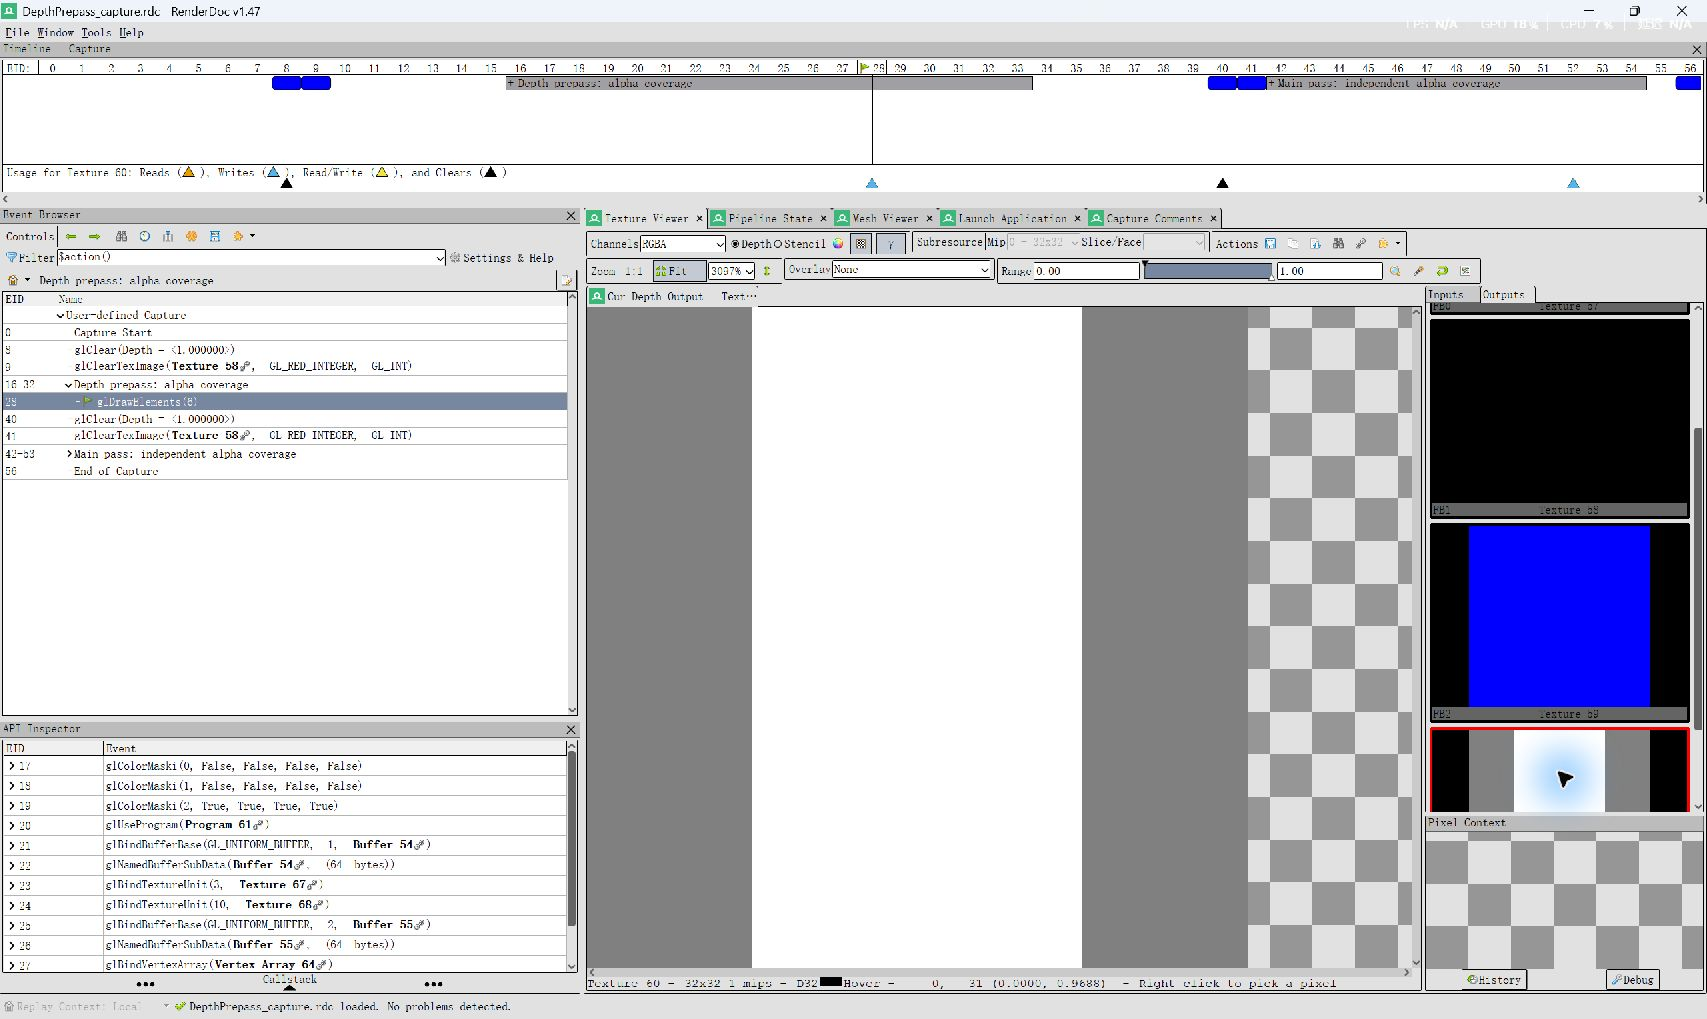
\includegraphics[width=\linewidth]{../../../output/captures/renderdoc-eid28-depth.jpg}
\caption{选中事件编号 EID 28 的深度预传递，Texture 60 为 D32 深度附件；两侧灰色为写入区域，中间白色保留清屏深度}
\end{figure}

回放定位到两次六索引绘制：EID 28 为深度预传递，EID 52 为主绘制。两者使用同一深度附件，中间有独立清屏。下表通过 RenderDoc 的 PickPixel 读取，坐标原点为左上，均位于 $y=16$。

\begin{tabularx}{\textwidth}{L{4.4cm}YYY}
\toprule
事件与附件 & $x=4$ & $x=12$ & $x=28$ \\
\midrule
EID 28，深度 & 0.5 & 1.0 & 0.5 \\
EID 52，深度 & 0.5 & 1.0 & 0.5 \\
EID 28，实体 ID & -1 & -1 & -1 \\
EID 52，实体 ID & 42 & -1 & 42 \\
\bottomrule
\end{tabularx}

全部 1024 个像素也已核对，两次绘制后的深度数据逐字节相同。512 个像素为 0.5，其余为 1.0。预传递不写实体 ID，因此全部保留 -1。主绘制在保留区域写入 42。六组自动测试另行覆盖更多开关组合。

捕获中还有 14 条信息消息和 1 条 NVIDIA 驱动性能提示：EID 28 的顶点着色器依据 GL 状态重新编译。回放开启 API 验证后只有 3 条信息消息，未报致命错误。尚未测量该重编译的持续时间和重复频率，不能写成零告警或已找到性能瓶颈。

\note{原始捕获：\path{output/captures/DepthPrepass_capture.rdc}，59936 字节。SHA-256 前缀为 \code{3dcc81ca9eb3ba44}，完整值与回放记录见同目录 manifest.json、replay-results.json。尚未测量 GPU 耗时。}


\newpage
\section{尚需单独验证的画面行为}
\subsection{SSAO 在屏幕边缘会减弱}
SSAO 遇到屏幕外样本时跳过累加，最后仍除以全部样本数。屏幕边缘遮蔽会减弱。本轮没有改成按有效样本数归一化，也没有做边缘场景的图像对比。
\loc{RedflagForge/assets/shaders/SSAO.glsl}

\subsection{RSM 历史仍可能混入旧表面}
当前深度用于还原世界位置，再投影到上一帧，历史颜色限制到当前邻域范围。这里没有运动矢量，也没有上一帧深度拒绝。移动物体和新露出的表面仍可能混入错误历史，应称为 RSM 历史混合，不能写成完整 TAA 或已解决拖影。
本次另修正上一帧位置超出近远裁剪面却仍采历史的问题。测试中本帧为 0.25，错误历史曾把结果混成约 0.7。现在裁剪范围外保留 0.25，合法位置仍正常混合。它检查投影范围，没有比较前帧实际表面的深度。
固定 128 点取前 N 个而缩小半径的问题已在第 \ref{sec:rsm-energy} 节修正。这项修改与历史是否来自同一表面是两个问题，不能把采样范围修正当作消除了拖影。
\loc{RedflagForge/assets/shaders/RSMTemporalResolve.glsl}

\subsection{玻璃保留几何，不等于半透明已经实现}
删除猜测代码后，曾被隐藏的玻璃几何会保留。当前导入仍只有 Opaque 和独立 AlphaMap 的 Mask 约定。正确半透明显示需要明确导入规则，以及排序和绘制设计，不能靠名称判断代替。

\section{复查入口}
\begin{tabularx}{\textwidth}{L{4.3cm}Y}
\toprule
资料 & 用于核对什么 \\
\midrule
\source{https://registry.khronos.org/OpenGL-Refpages/gl4/html/glDeleteVertexArrays.xhtml}{Khronos OpenGL：对象删除} & VAO 删除 API 的语义。 \\
\source{https://learnopengl.com/Advanced-OpenGL/Blending}{LearnOpenGL：Blending} & 像素裁剪与半透明混合的区别。 \\
\source{https://github.com/baldurk/renderdoc/blob/v1.x/docs/window/pipeline_state.rst}{RenderDoc：Pipeline State} & 在选定绘制之后检查使用中的状态和资源。 \\
\source{https://github.com/baldurk/renderdoc/blob/v1.x/docs/how/how_inspect_pixel.rst}{RenderDoc：像素检查} & 对照正确的附件、层级和实际像素值。 \\
项目测试与旧开发日志 & 本文具体故障、实现及验证范围的证据。 \\
\bottomrule
\end{tabularx}

\subsection{工具核查边界}
RenderDoc MCP 0.3.0 通过 stdio 读取到相同的两次绘制，事件编号与官方回放一致。但它的 get\_log 返回空列表，并未覆盖原捕获中的驱动诊断，因此仍以 replay-results.json 保存的消息为准。

另一次离屏 Qt 抓图漏掉原生 GPU 视图区，得到黑块，已作为截图失败记录，未收入文档。这不表示渲染输出为黑。最终采用实际窗口截图，数值由独立回放核对。两次工具核查分别记录在 \path{output/captures/mcp-check.json} 与 \path{gui-capture.json}。

更新本文时保留出错输入、定位过程、修复代码和复测结果。没有复现的旧问题继续保留证据限制。新截图须记录捕获文件、事件和附件，不能只留下没有上下文的画面。

\newpage
\section{代表性源码对照}
下面只节选决定行为的真实代码，省略无关上下文。修改前来自注明的提交，修改后来自本轮工作树或历史修复提交。短片段用于解释错误，完整生命周期仍应回到函数中核对。

\subsection{Mask：选择一项不等于三项相乘}
位置为 \path{RedflagForge/assets/shaders/Depth_Prepass.glsl} 的片元 main。修改前取自 \rev{1a168c3}，有透明度图时完全不使用底色因子的 alpha，也不读取底色贴图 alpha。

\textbf{修改前}
\begin{Code}
float alpha = u_UseAlphaMap == 1
    ? texture(u_AlphaMap, v_TexCoord).r
    : u_BaseColor.a;
if (alpha < u_AlphaCutoff)
    discard;
\end{Code}

\textbf{本轮修正}
\begin{Code}
float alpha = u_BaseColor.a;
if (u_UseBaseColorMap == 1)
    alpha *= texture(u_BaseColorMap, v_TexCoord).a;
if (u_UseAlphaMap == 1)
    alpha *= texture(u_AlphaMap, v_TexCoord).r;
if (alpha < u_AlphaCutoff)
    discard;
\end{Code}

修改还包括 C++ 上传底色图及使用开关，不能只改公式而不提供输入。DepthPrepassTests 独立清屏比较两次绘制。RenderDoc 的 EID 28 与 EID 52 进一步确认当次数据和 1024 个像素覆盖一致。Shadow 与 RSM 的覆盖由另一个测试验证，不由这张旧捕获推断。

\subsection{视锥剔除：保留光源仍需要的命令}
修改前取自同一提交的 Renderer3D::DrawMesh 材质重载。相机剔除后直接返回，Shadow 和 RSM 再也取不到这条命令。
\begin{Code}
if (CullMesh(*mesh, transform)) { s_Data.Stats.CulledCount++; return; }
s_Data.DrawCommands.push_back({ mesh, transform, material, entityID });
\end{Code}

本轮统一在 SubmitMesh 记录主相机可见性，先保留命令。
\begin{Code}
bool culled = CullMesh(*mesh, transform);
if (culled)
    s_Data.Stats.CulledCount++;
s_Data.DrawCommands.push_back({ mesh, transform, material, entityID, culled });
\end{Code}

随后只有相机预传递和主绘制筛掉 CameraCulled，光源阶段仍使用完整队列。Renderer3DTests 用相机外、光源内的四边形核对这一区别。
\loc{Redflag/src/Redflag/Renderer/Renderer3D.cpp}

\newpage
\section{历史源码对照：空批次重画旧数据}
提交 \rev{e80839c} 前，Renderer2D::EndScene 即使索引数量为零，也计算上传大小后调用 Flush。下段取自该提交的父版本，保留实际调用。

\textbf{修改前：EndScene 无条件提交}
\begin{Code}
uint32_t dataSize = (uint32_t)((uint8_t*)s_Data.QuadVertexBufferPtr -
    (uint8_t*)s_Data.QuadVertexBufferBase);
s_Data.QuadVertexBuffer->SetData(s_Data.QuadVertexBufferBase, dataSize);
Flush();
\end{Code}

空批次为什么仍会画出内容，还要继续查到当时 OpenGLRendererAPI::DrawIndexed。这里零数量表示使用整个索引缓冲，并不表示零次绘制。
\begin{Code}
uint32_t count = indexCount ? indexCount : vertexArray->GetIndexBuffer()->GetCount();
glDrawElements(GL_TRIANGLES, count,GL_UNSIGNED_INT,nullptr);
\end{Code}

\textbf{历史修正：有本批次索引才提交}
\begin{Code}
if (s_Data.QuadIndexCount > 0)
{
    uint32_t dataSize = (uint32_t)((uint8_t*)s_Data.QuadVertexBufferPtr -
        (uint8_t*)s_Data.QuadVertexBufferBase);
    s_Data.QuadVertexBuffer->SetData(s_Data.QuadVertexBufferBase, dataSize);
    Flush();
}
\end{Code}

这条判断放在拥有本批次计数的 2D 提交处，避免把空批次交给“零表示全部”的底层接口。它解释了旧缓冲为何有机会再次被读取，比只说“浮点误差”或“清屏有问题”更具体。

本轮核对了修复前后的完整调用链，原提交没有保存失败截图，也没有当时的自动测试日志。当前代码仍保留按有效数量提交的处理，但未补这项专门的空帧切换回归，不能把源码解释写成已重新复现。
\loc{Redflag/src/Redflag/Renderer/Renderer2D.cpp}
\loc{Redflag/src/Platform/OpenGL/OpenGLRendererAPI.cpp}

\end{document}
